\documentclass[paper=letter,11pt]{scrartcl}

\KOMAoptions{headinclude=true, footinclude=false}
\KOMAoptions{DIV=14, BCOR=5mm}
\KOMAoptions{numbers=noendperiod}
\KOMAoptions{parskip=half}
\addtokomafont{disposition}{\rmfamily}
\addtokomafont{part}{\LARGE}
\addtokomafont{descriptionlabel}{\rmfamily}
%\setkomafont{pageheadfoot}{\normalsize\sffamily}
\setkomafont{pagehead}{\normalsize\rmfamily}
%\setkomafont{publishers}{\normalsize\rmfamily}
\setkomafont{caption}{\normalfont\small}
\setcapindent{0pt}
\deffootnote[1em]{1em}{1em}{\textsuperscript{\thefootnotemark}\ }


\usepackage{amsmath}
\usepackage[varg]{txfonts}
\usepackage[T1]{fontenc}
\usepackage{graphicx}
\usepackage{xcolor}
\usepackage[american]{babel}
% hyperref is needed in many places, so include it here
\usepackage{hyperref}

\usepackage{xspace}
\usepackage{multirow}
\usepackage{float}


\usepackage{braket}
\usepackage{bbm}
\usepackage{relsize}
\usepackage{tcolorbox}

\def\ketY{\ensuremath{\ket {\Psi}}}
\def\iGeV{\ensuremath{\textrm{GeV}^{-1}}}
%\def\mp{\ensuremath{m_{\textrm{proton}}}}
\def\rp{\ensuremath{r_{\textrm{proton}}}}
\def\me{\ensuremath{m_{\textrm{electron}}}}
\def\aG{\ensuremath{\alpha_G}}
\def\rAtom{\ensuremath{r_{\textrm{atom}}}}
\def\rNucl{\ensuremath{r_{\textrm{nucleus}}}}
\def\GN{\ensuremath{\textrm{G}_\textrm{N}}}
\def\ketX{\ensuremath{\ket{\vec{x}}}}
\def\ve{\ensuremath{\vec{\epsilon}}}


\def\ABCDMatrix{\ensuremath{\begin{pmatrix} A &  B  \\ C  & D \end{pmatrix}}}
\def\xyprime{\ensuremath{\begin{pmatrix} x' \\ y' \end{pmatrix}}}
\def\xyprimeT{\ensuremath{\begin{pmatrix} x' &  y' \end{pmatrix}}}
\def\xy{\ensuremath{\begin{pmatrix} x \\ y \end{pmatrix}}}
\def\xyT{\ensuremath{\begin{pmatrix} x & y \end{pmatrix}}}

\def\IMatrix{\ensuremath{\begin{pmatrix} 0 &  1  \\ -1  & 0 \end{pmatrix}}}
\def\IBoostMatrix{\ensuremath{\begin{pmatrix} 0 &  1  \\ 1  & 0 \end{pmatrix}}}
\def\JThree{\ensuremath{\begin{pmatrix}    0 & -i & 0  \\ i & 0  & 0 \\ 0 & 0 & 0 \end{pmatrix}}} 
\def\JTwo{\ensuremath{\begin{bmatrix}    0 & 0 & -i  \\ 0 & 0  & 0 \\ i & 0 & 0 \end{bmatrix}}}
\def\JOne{\ensuremath{\begin{bmatrix}    0 & 0 & 0  \\ 0 & 0  & -i \\ 0 & i & 0 \end{bmatrix}}}
\def\etamn{\ensuremath{\eta_{\mu\nu}}}
\def\Lmn{\ensuremath{\Lambda^\mu_\nu}}
\def\dmn{\ensuremath{\delta^\mu_\nu}}
\def\wmn{\ensuremath{\omega^\mu_\nu}}
\def\be{\begin{equation*}}
\def\ee{\end{equation*}}
\def\bea{\begin{eqnarray*}}
\def\eea{\end{eqnarray*}}
\def\bi{\begin{itemize}}
\def\ei{\end{itemize}}
\def\fmn{\ensuremath{F_{\mu\nu}}}
\def\fMN{\ensuremath{F^{\mu\nu}}}
\def\bc{\begin{center}}
\def\ec{\end{center}}
\def\nus{$\nu$s}

\def\adagger{\ensuremath{a_{p\sigma}^\dagger}}
\def\lineacross{\noindent\rule{\textwidth}{1pt}}

\newcommand{\multiline}[1] {
\begin{tabular} {|l}
#1
\end{tabular}
}

\newcommand{\multilineNoLine}[1] {
\begin{tabular} {l}
#1
\end{tabular}
}



\newcommand{\lineTwo}[2] {
\begin{tabular} {|l}
#1 \\
#2
\end{tabular}
}

\newcommand{\rmt}[1] {
\textrm{#1}
}


%
% Units
%
\def\m{\ensuremath{\rmt{m}}}
\def\GeV{\ensuremath{\rmt{GeV}}}
\def\pt{\ensuremath{p_\rmt{T}}}


\def\parity{\ensuremath{\mathcal{P}}}

\usepackage{cancel}
\usepackage{ mathrsfs }
\def\bigL{\ensuremath{\mathscr{L}}}

\usepackage{ dsfont }



\usepackage{fancyhdr}
\fancyhf{}

%\documentclass[margin,line]{res}
\usepackage{braket}
\usepackage{bbm}
\usepackage{relsize}

\def\ketY{\ensuremath{\ket {\Psi}}}
\def\iGeV{\ensuremath{\textrm{GeV}^{-1}}}


\def\ABCDMatrix{\ensuremath{\begin{pmatrix} A &  B  \\ C  & D \end{pmatrix}}}
\def\xyprime{\ensuremath{\begin{pmatrix} x' \\ y' \end{pmatrix}}}
\def\xyprimeT{\ensuremath{\begin{pmatrix} x' &  y' \end{pmatrix}}}
\def\xy{\ensuremath{\begin{pmatrix} x \\ y \end{pmatrix}}}
\def\xyT{\ensuremath{\begin{pmatrix} x & y \end{pmatrix}}}

\def\IMatrix{\ensuremath{\begin{pmatrix} 0 &  1  \\ -1  & 0 \end{pmatrix}}}
\def\IBoostMatrix{\ensuremath{\begin{pmatrix} 0 &  1  \\ 1  & 0 \end{pmatrix}}}
\def\JThree{\ensuremath{\begin{pmatrix}    0 & -i & 0  \\ i & 0  & 0 \\ 0 & 0 & 0 \end{pmatrix}}} 
\def\JTwo{\ensuremath{\begin{bmatrix}    0 & 0 & -i  \\ 0 & 0  & 0 \\ i & 0 & 0 \end{bmatrix}}}
\def\JOne{\ensuremath{\begin{bmatrix}    0 & 0 & 0  \\ 0 & 0  & -i \\ 0 & i & 0 \end{bmatrix}}}
\def\etamn{\ensuremath{\eta_{\mu\nu}}}
\def\Lmn{\ensuremath{\Lambda^\mu_\nu}}
\def\dmn{\ensuremath{\delta^\mu_\nu}}
\def\wmn{\ensuremath{\omega^\mu_\nu}}
\def\be{\begin{equation*}}
\def\ee{\end{equation*}}
\def\bc{\begin{center}}
\def\ec{\end{center}}
\def\nus{$\nu$s}
\def\nue{\ensuremath{\nu_e}}
\def\numu{\ensuremath{\nu_\mu}}
\def\nutau{\ensuremath{\nu_\tau}}
\def\nualpha{\ensuremath{\nu_\alpha}}
\def\nuone{\ensuremath{\nu_1}}
\def\nutwo{\ensuremath{\nu_2}}
\def\nuthree{\ensuremath{\nu_3}}
%\def\xMu{\ensuremath{x^\mu}

\usepackage{fancyhdr}

\fancyhf{}
\lhead{\Large 33-444} % \hfill Introduction to Particle Physics \hfill Spring 2019}
\chead{\Large Introduction to Particle Physics} % \hfill Spring 2019}
\rhead{\Large Spring 2019} % \hfill Introduction to Particle Physics \hfill Spring 2019}

\begin{document}
\thispagestyle{fancy}

\begin{center}
{\huge \textbf{Lecture 36}}
\end{center}

{\fontsize{14}{16}\selectfont

\textbf{\underline{OK left off discussing how 2-state mixing describes atmospheric \nus}} 

Turns out that two flavour $\nu$ oscillations also explains the solar $\nu$ oscillations very well. 
(More complicated b/c of matter effects that we are not going to talk about)

$\Delta m^2 \sim 10^{-4} eV^2$ 

This means we have another $\Delta m^2$ that explains how \nue s disappear, with a large mixing angle. 
Can I do an experiment to test that ?

If,  $\Delta m^2 \sim 10^{-4} eV^2$,  for a 1 GeV $\nu$, oscillation length is $10^4$ km. 

Idea to do an experiment with reactor \nus.
$E_\nu \sim 5 MeV \Rightarrow $ baselines of 100 km. 

Describe Kamland. 

Confirms the picture that you get out of the solar \nus.

\noindent\rule{\textwidth}{1pt}

Picture that we have constructed is pretty simple

\underline{Atmospheric Oscillations:}
\be
\Delta m^2 \sim 10^{-3} eV^2
\ee
\be
\numu \longleftrightarrow \nutau
\ee
\bc
Large Mixing Angle
\ec

\underline{Solar Oscillations:}
\be
\Delta m^2 \sim 10^{-4} eV^2
\ee
\be
\nue \longleftrightarrow \numu,\nutau
\ee
\bc
Large Mixing Angle
\ec

We know we have three \nus, these results are all with 2 state toy. 
How do we make this into a coherent picture. 
Why doesn't this work so well, even though we have 3 \nus?

Answer is the folllowing:
 this is a two frequency phenomenon or there are two relevant oscilation lengths.
 one is long and the other is short. 

Atmosphereic is short / Solar is long. 
Ratio between them is factor of $\sim$30.

So even though you have \nue\ going to \numu\ and \nutau\ from the solar picture , that doesnt screw up the atmospheric picture very much beacues the atmosphere lenghth scales are such that you dont get to see the solar oscillations, the wavelength is too long. 

For the solar \nus\ you can ask how come the \nue s cant see the other oscillation length? fair question. 
The reason you cant see that is there is a mixing angle that is small. 

\noindent\rule{\textwidth}{1pt}

\textbf{This is what we knew $\sim 10$ years ago.}

Knew this picture worked well, knew why the 2flavour approximation was so good. 
Hierarchy of oscillation scales. 
Turns out that the \nue s didnt get to see the fast oscillation bc of a small mixing angle. 

The next challenge in $\nu$-physics was how do we get to see this effect or can we get to see \nue s participating with the atmospheric mixing frequency. 
This was the big question in $\nu$-physics 10 years ago.
Came up with lots of different ways do it, best way is the reactor expirment. 
Did three of them just to be sure. 
Looking for a potentially tiny effect (not sure how small the mixing is, knew it was reasonably small) 

\bc
Daya Bay / 
RENO  /
Double Chooz
\ec

Turns out it was an 8\% effect. (Larger than expected)

\underline{These are all disapearnce experiments.}
Start out with a numebr of \nus\ measure a deficit after 1km. 
Need to know how much you start out with. 
This is that makes these experiments hard.
Very hard to predict how many \nus\ come from a reactor at the few percent level. 
So you do whats called a two dector experiment. 

\be
\nue \rightarrow \textrm{ disappears }
\ee
\bc
Small Mixing Angle
\ec

This explains lots of thingsn
- why the two systemss separate in a way that makes life easy to interpret the data

This is what weve been able to do and where we are today. 
Have actually done a little better, have seen $\numu \rightarrow \nue$ with the same small angle. Taking data now (Nova/T2K)


\noindent\rule{\textwidth}{1pt}

\underline{\textbf{Putting it all together}}

%\be
%\begin{pmatrix} \nue \\ \numu \\ \nutau \end{pmatrix} = \begin{pmatrix} U_{e1} & U_{e2} & U_{e3}  \\ U_{\mu 1} & U_{\mu 2} & U_{\mu 3}  \\ U_{\tau 1} & U_{\tau 2} & U_{\tau 3}  \end{pmatrix} \begin{pmatrix} \nuone \\ \nutwo \\ \nuthree \end{pmatrix} 
%\ee

What havent we determined yet ?

\textbf{Mass ordering:}  Inverted vs Normal ordering. 

\begin{figure}[h!]
\centering
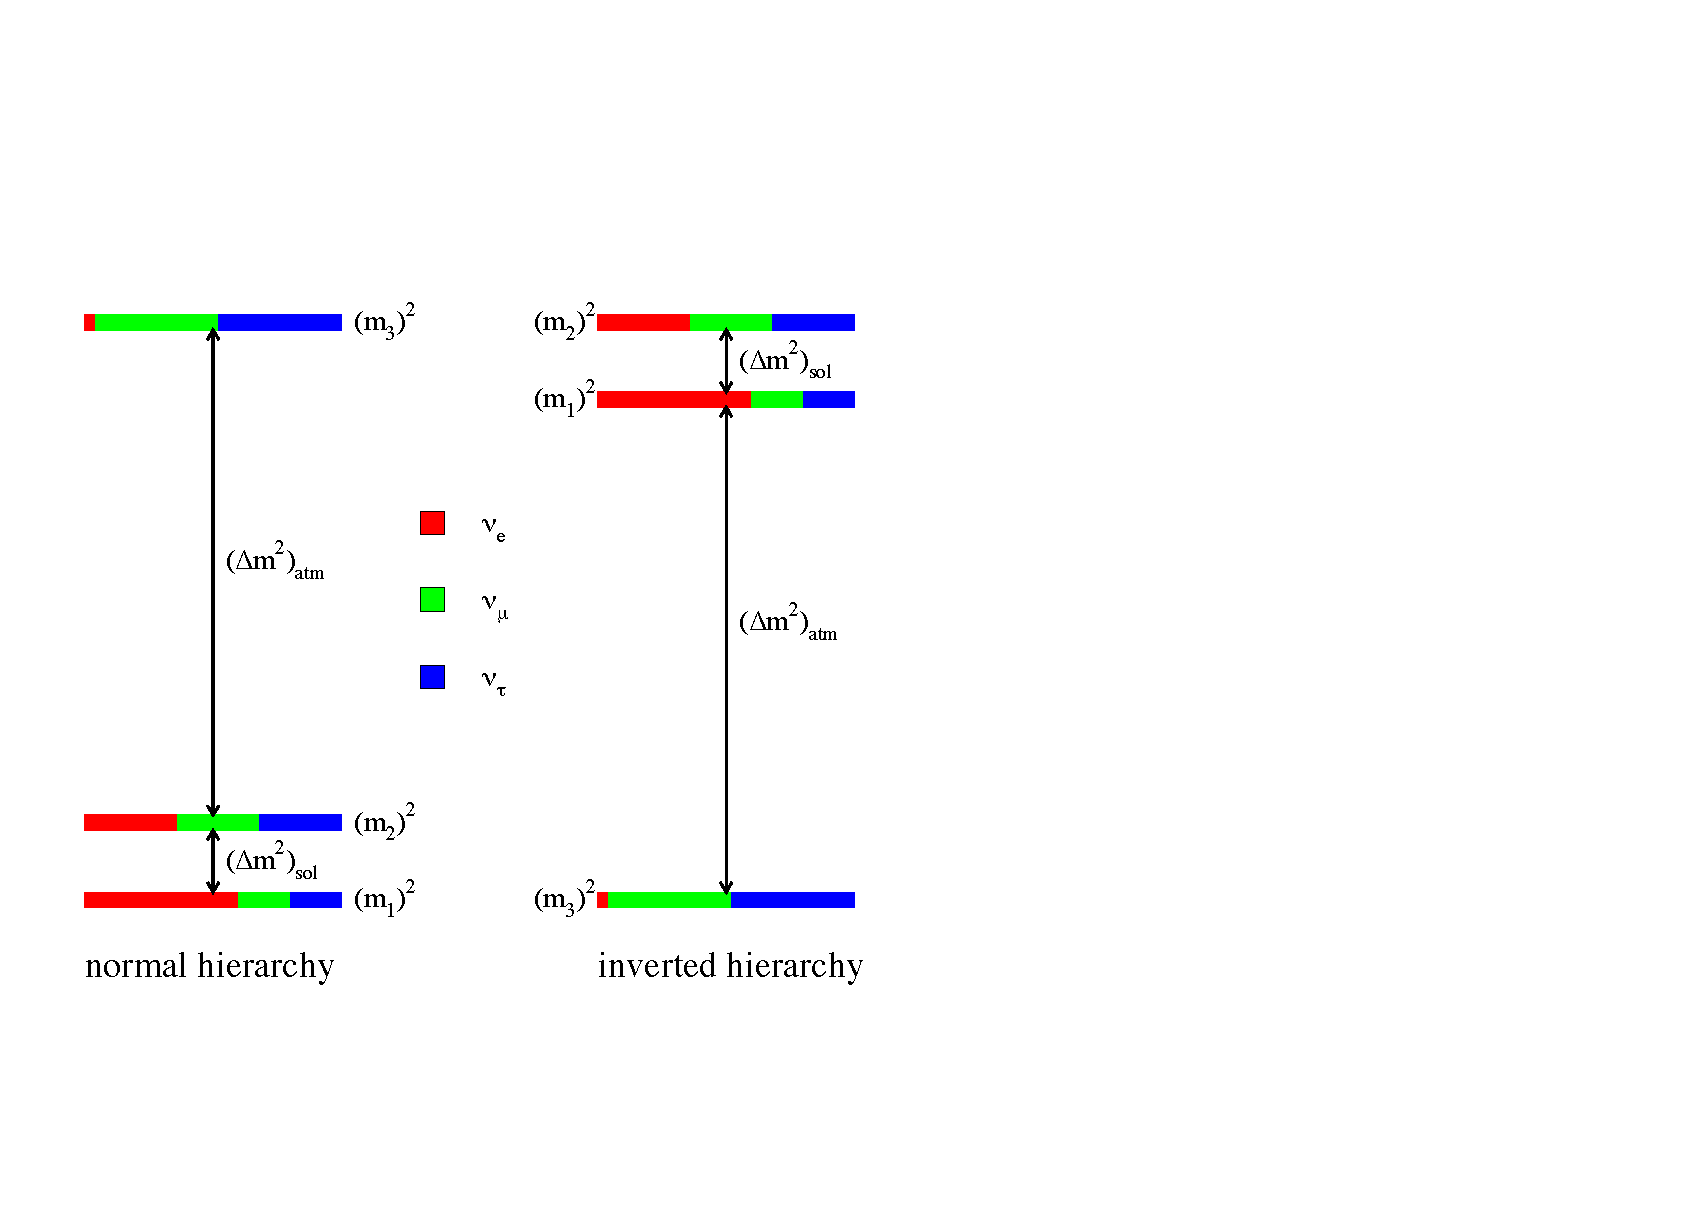
\includegraphics[width=0.8\textwidth]{./NuMass.pdf}
\end{figure}

How do we think we are going to measure the $\nu$\ mass hierarchy?

Two ways: 
  - Most obvious way the hardest:  
  There are actually 3 oscillation lengths.       
  The differnces are diffenrent. If we could see all three would 
  Juno experiment in China is aimed at doing this. 
   Hard: Need distance and very good resolution short 
          Really big dector with very good resolution (These are usually competing requirements) 

  - Matter effects. 
      \nue\ behaves differently in matter (there are electrons around) 
      Nova 

\noindent\rule{\textwidth}{1pt}

\textbf{CP Violation:}  Comments 
   $70^{o}$ in quark sector
   theta CP $\sim0  < 10^{-10}$

\noindent\rule{\textwidth}{1pt}

\textbf{$\nu$ masses}

Want to measure the $\nu$ masses

-Possible that the lightest is very nearly massless . \\
-Possible that all the masses are the same and the splittings are very small.

From a physics point of view this looks very different.
\bc
 Degenerate (split by a little bit)  vs  hierarchical 
\ec
The physics that might live behind that is different.

Measuring the masses has nothing to do with mixing: Cosmology / Particle physics 
 
beta decay spectra: KATRIN /  $10^{-12}$ / shape of the spectrum

\noindent\rule{\textwidth}{1pt}

\textbf{``Dirac vs Marani``} 

How many $\nu$ DoFs ?  4 DoF  or 2 DoF? 

What prevents us from telling the differnece ?

\textbf{If $m_e$ = 0}, we have two very different fields L and R completely unrelated to one another.
You would never connect them to one another. 
Only reason they are coupled is throught the mass, there is an interaction that can transform a left-handed electron into a right-handed one.
That is how they are ``combined'' into a dirac fermion.

\textbf{If $m_\nu$ = 0},
The left-handed nu and the ``would-be'' right-handed nu would be completely differnet particles. 
The right-handed nu in this scenerio is a completely useless particle (no interactiosn at all)
The right-handed nu only manifisted itself if $m_\nu$ != 0

They way you tell this is through neutrino-less double beta decay

 Z -> Z' + e + e 

 Z -> Z' + e + e  + nu + nu (very rare) has been observed (two neutrons decay at the same time) 


\noindent\rule{\textwidth}{1pt} 

\textbf{Why are people excited about $\nu$ physics? }

Have discovered that $\nu$ masses exist. 
Most amazing thing is that they are really small. 
Small compared to any masses you can think of. 

\begin{figure}[h!]
\centering
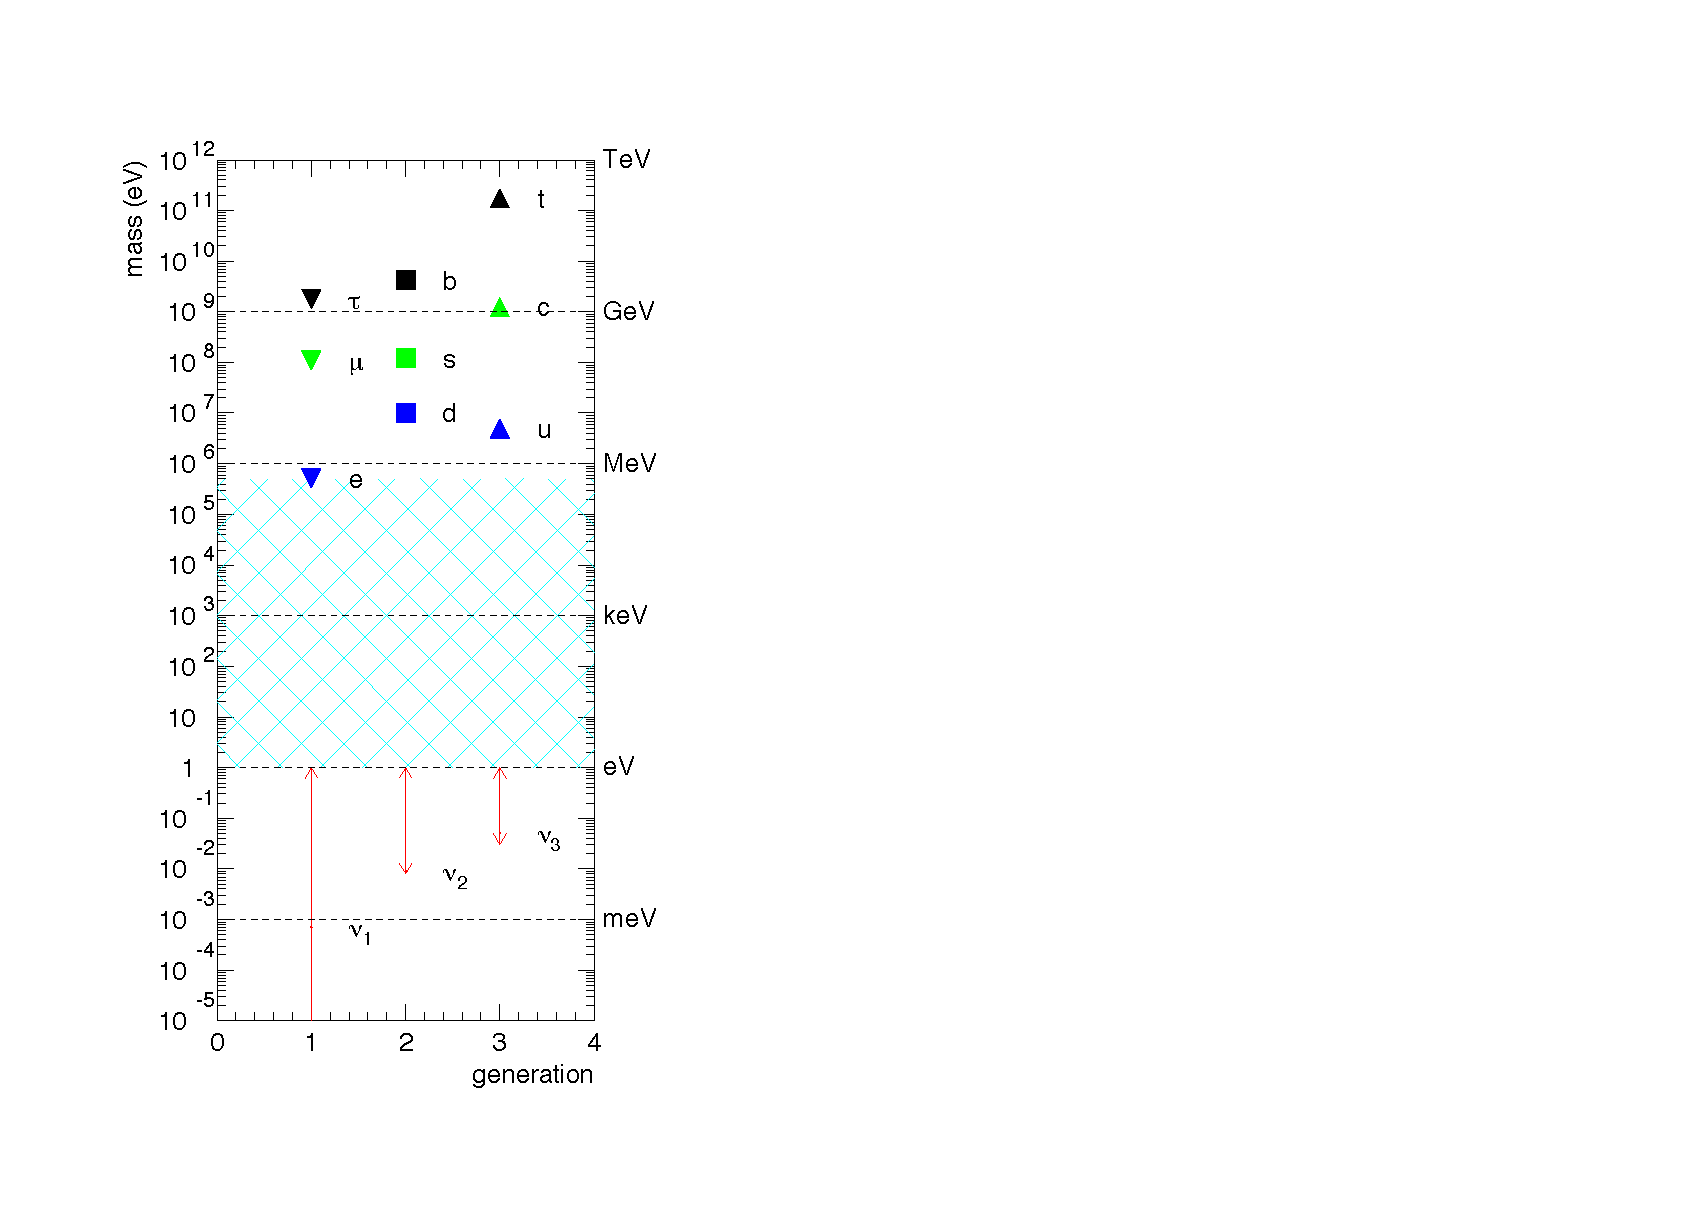
\includegraphics[width=0.5\textwidth]{./NuMass2.pdf}
\end{figure}


One of the biggest embarassement in Particle physics. 
log plot.   Masses very different. 
All fundamental as far as we can tell. 
Masses span 16 orders of magnitude. 
nus are responsible for more than 1/2 that span. 

Spent a long time trying to understand why other fermion masses are so differenet. 
Havent gotten anywhere. 
Now \nus\ live way down here.

Another strange thing, the charged fermion mass range is nicely populated. 
So every once in a while if your doign physics vs E you would run into a new fermion. 
Life is interesting. 
Particle physics in 60 and 70s. 

The gap between the heaviest $\nu$ and the electron is bigger than the differnece between the electron and the top quark mass. 
What does any of this mean ? 
We have no idea.
Looks like something important.
So a lot of time is spent thinking about this.

Why are we excited about $\nu$ masses? 
\begin{itemize}
\item[-] Very small
\item[-] qualtiatively different (?)
\end{itemize}

Everything is speculative...

%- Majorana fermions \\
%- In SM $m_\nu$ = 0.  (something we get very excited about) 

(Why did we believe $m_\nu$ = 0 in the SM ?)

Given the SM how do I give nus a mass ?

$m_\nu$s> 0 mean new DoF.


Q u d L e  + H + SU(3) x SU(2) x U(1)

Whats interesting about that is if this is all you know you can write down the lagrangian. 

Unabmigious Langrangian,  this lagrangian give you $m_\nu$ = 0.

IF you want to make $m_\nu$ > 0, somethign in this line has to change. 

One way, Assume that the SM is an effective theory. 
  Can keep playing the same game and write down higher dimensional operators. 

  Start at dimension 5. 
  Turns out there is only one dim-5 operator. 


 (LH)(LH)/M + P(dim-6) 

What does this operator do ?
IF M is high enough, this operator does only one thing. 

H gets a vev:   $L \sim  v^2 \nu^2 / M   = m_\nu  \nu^2$

This theory predicts that the first thing you should see is a non-zero $m_\nu$. 

 $m_\nu = v^2 / M$

what makes this intersting is that this mass is parameterically differnet form charged fermion masses, 

 $m_l \propto v$   whereas $m_\nu \propto v^2$

This would ``explain'' why the $m_\nu$s are qualitatively differnet. 

So you could have written down this theory,   predict that $m_\nu$>0 is first sign of new phsyics, predict that $m_\nu$s are very small, and will predict that they are majorana masses. 

Very old idea (wienberg '79) 

Most everyone is willing to bet that this is how $m_\nu$s happen. 
Sounds so plausible, 

Required new DoF and some new Mass scale M.  
Could be very heavy.
$L \sim 10^{14}$ GeV 


This is one general idea. 

\noindent\rule{\textwidth}{1pt} 

Lets talk about another general idea. 

More mondane, but will try convince you why this is intersting. 

Well talk next week the plank scale, L sim $10^{14}$ GeV way below the $m_{plank}$. 

Other option is to mess around with the particle content in the SM.
 Two options, add stuff to the fermion content or add stuff to the Higgs content. 
 The higgs part is pretty easy. 

Add a triplet. 

LTL majorana mass,  private higgs to the nus. 
The triplet vev is very small so its probably OK. 

All kinds of problems with the triplet. 
T has lepton number, if lepton number symetry is not explictly broken it becomes can do this by adding new particles. 


Other way is the way everyone thinks of. 

Include Right-handed nus,   $\nu^R$. 

dont interact / no gauge Quantum numbers. 

$L \supset  y LHv $

after EWSB, 
  $m_\nu  \sim y v$    ($y \sim10^{-12}$ not disallowed,  but weird )
  ($y_e$ is $\sim10^{-6}$ lived with that for a while)

Why is this model interesting? 
(Theory prejuduge comes into play)

Could right down SM with: 
Q u d L e  + H + SU(3) x SU(2) x U(1)
Stopped at the renormalizible level. 

IF you add nu and play the same game, 

$L \supset  y LHv$  is not the L that you get,  your missing a term. 

Can also write down a term like $L \supset - M/2 \nu \nu$. 
(This is allowed and is a relavent operator, adding a new relavent operator.  
  New mass scale in the SM. (no naturalness problem) 

Qualtitatively different from the L we had before. 
Question becomre if you allow for $\nu_R$ should allow for the possibility that mass terms exisit. 
Depending on what those mass term are the phenomelogy is very different. 

What happens in generall dont know how many $\nu_R$s should exist. (Maybe 3) 
(Need at least 2) 
L predicts the existance of 6 nutrual objects, masses majoranan fermions.

If $M >> yxv$, then you can integrate out the heave neutronio,

$L \sim y^2 LH^2 / M$  (Weinberg operator) 
Three light + three heavy. 

M > eV / all OK except cosmology 
  > MeV / cosmology OK

=================

M = 0, allowed to do this. 
IF the L has lepton number symmetry this number is exactly 0. 
 => Lepton number is a fundamental symmetry of nature. 

Very differnt then how we look at lepton number today. 
In the SM, no where do I ask for Lepton Number (or Baryon Number) conservation. 
It just happens. 


  

}
\end{document}


